\documentclass[border=2mm]{standalone}
\usepackage{tikz}
\usetikzlibrary{calc}

\begin{document}

% Hình 1: ô x^2 là hình vuông
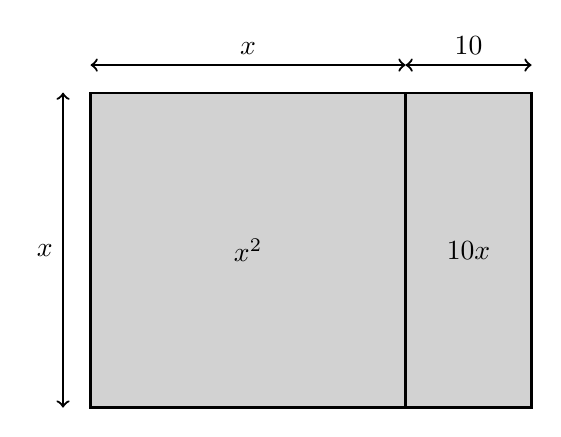
\begin{tikzpicture}
  % tham số hình học (đơn vị tikz mặc định: cm)
  \def\xside{4}   % cạnh ô vuông x^2 (biểu diễn "x")
  \def\tenw{1.6}  % bề rộng dải "10" (tùy chọn thị giác)
  \def\pad{0.35}

  % nền + khung
  \fill[gray!35] (0,0) rectangle (\xside+\tenw,\xside);
  \draw[thick] (0,0) rectangle (\xside+\tenw,\xside);
  \draw[thick] (\xside,0) -- (\xside,\xside);

  % nhãn trong các phần
  \node at (\xside/2,\xside/2) {$x^2$};
  \node at (\xside+\tenw/2,\xside/2) {$10x$};

  % mũi tên đo trên: x và 10
  \draw[<->,thick] (0,\xside+\pad) -- node[above] {$x$} (\xside,\xside+\pad);
  \draw[<->,thick] (\xside,\xside+\pad) -- node[above] {$10$} (\xside+\tenw,\xside+\pad);

  % mũi tên đo bên trái: x
  \draw[<->,thick] (-\pad,0) -- node[left] {$x$} (-\pad,\xside);
\end{tikzpicture}


\end{document}